%%    _____  _____
%%   |  __ \|  __ \    AUTHOR: Pedro Rivero
%%   | |__) | |__) |   ---------------------------------
%%   |  ___/|  _  /    DATE: November 10, 2021
%%   | |    | | \ \    ---------------------------------
%%   |_|    |_|  \_\   https://github.com/pedrorrivero
%%

\begin{frame}[allowframebreaks]{Quantum Fourier transform}

	The usual \textbf{Discrete Fourier Transform} (DFT) can be expressed as:

	\medskip

	\begin{align*}
	  \ket{j} \qra&
				\frac{1}{\sqrt{N}} \sum_{k=0}^{N-1} \exp[2\pi i \frac{jk}{N}] \ket{k} \\
	    =& \frac{1}{2^{n/2}} \sum_{k_{n-1}=0}^{1} \cdots \sum_{k_{0}=0}^{1}
	      \exp[2\pi ij \qty(\sum_{l=0}^{n-1} k_{l} 2^{l-n})]
	      \ket{\bin k_{n-1} \dots k_{0}} \\
	    =& \frac{1}{2^{n/2}} \sum_{k_{n-1}=0}^{1} \cdots \sum_{k_{0}=0}^{1}
	      \qty{ \bigotimes_{l=1}^{n} \exp[2\pi ij k_{n-l} 2^{-l}]
	      \ket{k_{n-l}} } \\
	    =& \frac{1}{2^{n/2}} \bigotimes_{l=1}^{n}
	      \qty{ \sum_{k_{n-l}=0}^{1} \exp[2\pi ij k_{n-l} 2^{-l}] \ket{k_{n-l}} }
	    = \frac{1}{2^{n/2}} \bigotimes_{l=1}^{n}
	      \qty{ \ket{0} + \exp[2\pi ij 2^{-l}] \ket{1} }
	\end{align*}

\break

	\begin{gather*}
		\ket{j} \ra
			\frac{
				\qty{\ket{0}+ e^{2\pi i \qty(\bin.j_{0})} \ket{1}} \otimes
				\qty{\ket{0}+ e^{2\pi i \qty(\bin.j_{1}j_{0})} \ket{1}} \otimes
				\cdots \otimes
				\qty{\ket{0} + e^{2\pi i \qty(\bin.j_{n-1}j_{n-2} \dots j_{0})} \ket{1}}
			}{2^{n/2}} \\[10pt]
		R_{k} \defeq \mqty[1 & 0 \\ 0 & e^{2\pi i/2^k}]
	\end{gather*}

	\vspace{-2em}

	\begin{center}
		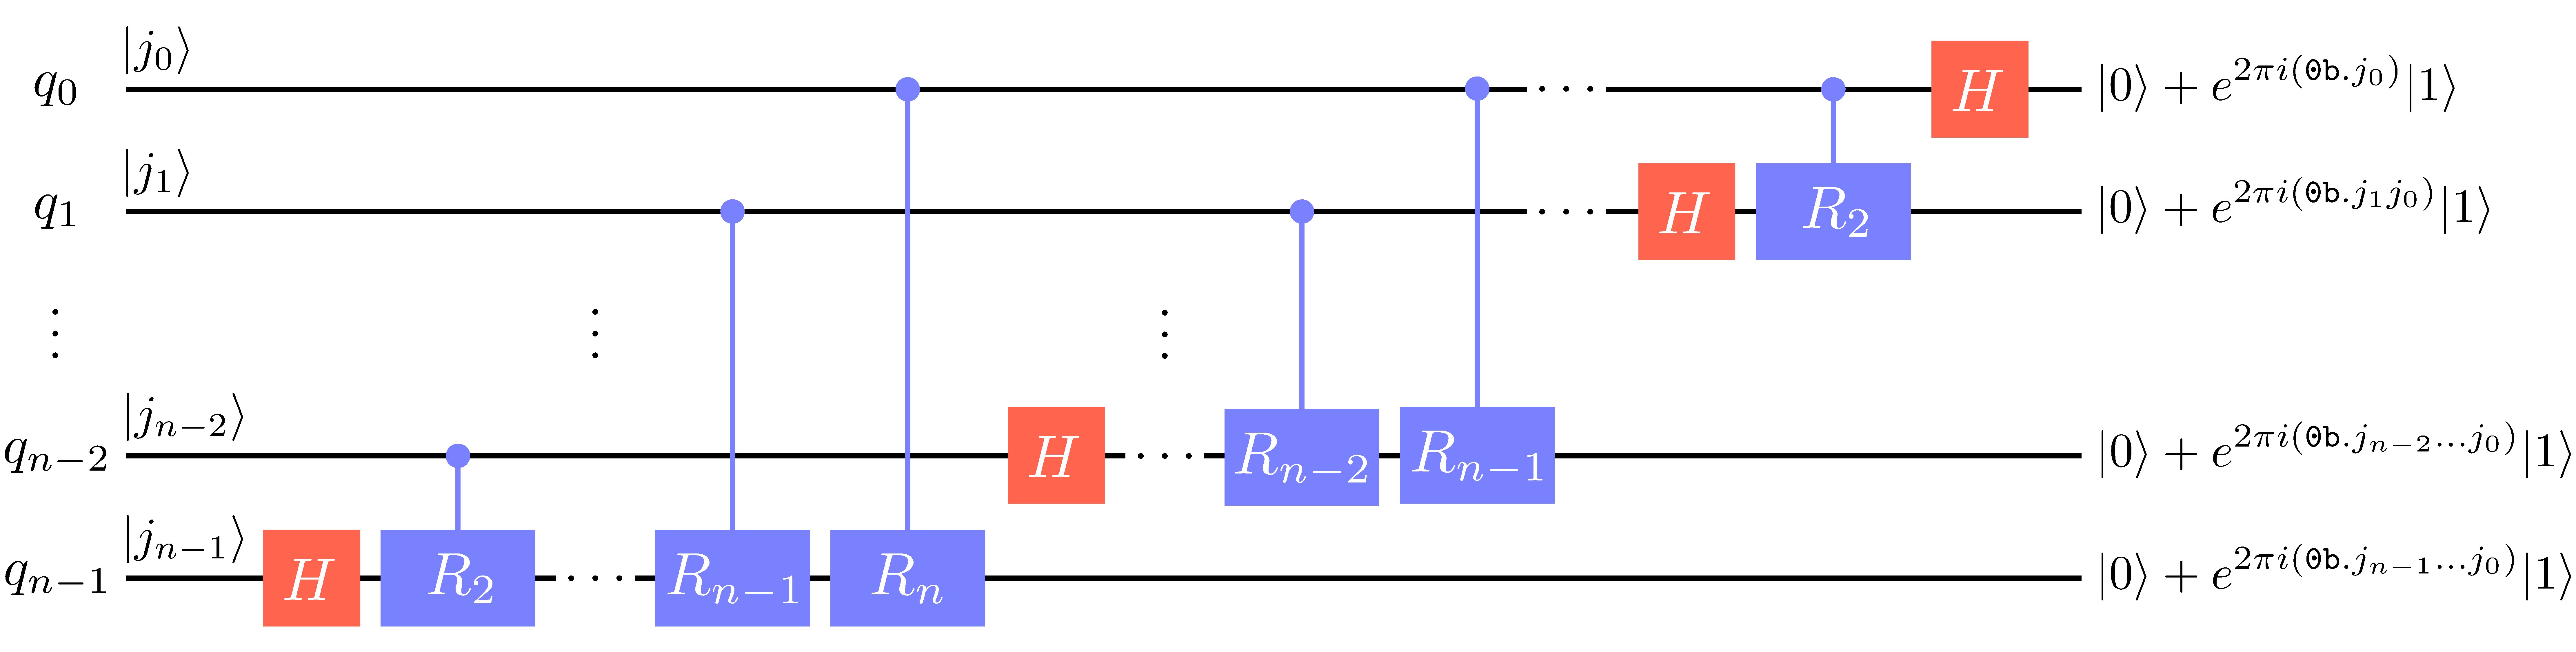
\includegraphics[width=.80\paperwidth]{Figures/quantum-background/quantum-fourier-transform}
	\end{center}

\break

	We can now compare the complexity of this algorithm with its best classical counterparts. This is done by counting the number of gates in the circuit, where we have to remember the final SWAP gates omitted in the representation.

	\begin{multicols}{2}
	\begin{centering}

		\underline{\textbf{FAST FOURIER TRANSFORM}}\\
		\medskip
		$N\log_2 N \equiv \Theta\qty(n2^n)$

		\columnbreak

		\underline{\textbf{QUANTUM FOURIER TRANSFORM}}\\
		\medskip
		$\sum_{k=1}^{n}k + \frac{n}{2} =
			\frac{n\qty(n+1)}{2} + \frac{n}{2} \equiv \Theta\qty(n^2)$

	\end{centering}
	\end{multicols}

	Nonetheless, this technique cannot be used directly for computing the target transform; since we do not know how to recover the individual amplitudes from the quantum states. On top of that, there is no efficient general method for preapring the states to be transformed. This is a great example of an algorithm that presents huge savings compared to its classical analogs, but which cannot be generally used as much as we would like to due to our inability to extract the desirerd information. In some instances however, we can profit from this method to great deeds ---mainly as part of bigger algorithms. An important application is \textbf{Shor's factoring algorithm}, which can be used for efficiently finding the prime decomposition of any given number.

\end{frame}
